\documentclass[aaspp]{article}

\usepackage[utf8]{inputenc}
\usepackage{txfonts}
\usepackage{rotating}
\usepackage{amssymb}
\usepackage{natbib}
\usepackage{varioref}
\usepackage{xspace}

%%Units
%\newcommand{\degr}{$^\circ$\xspace}

%Solar amounts
\newcommand{\ro}{R$_\odot$\xspace}
\newcommand{\mo}{M$_\odot$\xspace}
\newcommand{\zo}{Z$_\odot$\xspace}

\newcommand{\tc}{$\mathrm{\theta}^1\mathrm{C}$\xspace}

%Physical variables
\newcommand{\teff}{$\mathrm{T}_{\mathrm{eff}}$\xspace}
\newcommand{\te}{$\mathrm{T}_{\mathrm{e}}$\xspace}
\newcommand{\nelec}{$\mathrm{n}_{\mathrm{e}}$\xspace}

%This is necesary for the \ion command works
\DeclareRobustCommand\ion[2]{%
  \mbox{#1\kern0.2em%
    \smaller\rmfamily%
    \edef\@tempa{\@car#2\@nil}%
    \ifcat1\@tempa%
    \@Roman{#2}%
    \else%
    \uppercase{#2}%
    \fi}}
\newcounter{IonStage}
\DeclareRobustCommand\plainion[2]{\setcounter{IonStage}{#2}#1
  \Roman{IonStage}}
\DeclareRobustCommand\nodata{$\cdots$}
\newcommand{\smaller}{\small}

%This are my most used lines
\newcommand{\ha}{H$\alpha$\xspace}
\newcommand{\hb}{H$\beta$\xspace}
\newcommand{\hii}{\ion{H}{ii}\xspace}
\newcommand{\he}{\ion{He}{i}\xspace}
\newcommand{\sii}{[\ion{S}{ii}]\xspace}
\newcommand{\siip}{[\ion{S}{ii}]+\xspace}
\newcommand{\nii}{[\ion{N}{II}]\xspace}
\newcommand{\oi}{[\ion{O}{I}]\xspace}
\newcommand{\oii}{[\ion{O}{II}]\xspace}
\newcommand{\oiii}{[\ion{O}{III}]\xspace}
\newcommand{\neii}{[\ion{Ne}{II}]\xspace}
\newcommand{\lhe}{\ion{He}{I}$\lambda5876$\xspace}
\newcommand{\lsii}{[\ion{S}{II}]$\lambda6716$\xspace}
\newcommand{\lsiimas}{[\ion{S}{II}]$\lambda6716+\lambda6731$\xspace}
\newcommand{\lnii}{[\ion{N}{II}]$\lambda6583$\xspace}
\newcommand{\loi}{[\ion{O}{I}]$\lambda6300$\xspace}
\newcommand{\loii}{[\ion{O}{II}]$\lambda3727$\xspace}
\newcommand{\loiii}{[\ion{O}{III}]$\lambda5007$\xspace}

\newcommand{\R}{$\mathrm{R}$\xspace}

\begin{document}

%
%  These Macros are taken from the AAS TeX macro package version 4.0.
%  Include this file in your LaTeX source only if you are not using
%  the AAS TeX macro package and need to resolve the macro definitions
%  in the BibTeX entries returned by the ADS abstract service.
%
%  For more information on the AASTeX macro package, please see the URL
%	http://www.ferberts.com/AAS/aastex.html
%  For more information about ADS abstract server, please see the URL
%	http://adswww.harvard.edu/ads_abstracts.html
%

% Abbreviations for journals.  The object here is to provide authors
% with convenient shorthands for the most "popular" (often-cited)
% journals; the author can use these markup tags without being concerned
% about the exact form of the journal abbreviation, or its formatting.
% It is up to the keeper of the macros to make sure the macros expand
% to the proper text.  If macro package writers agree to all use the
% same TeX command name, authors only have to remember one thing, and
% the style file will take care of editorial preferences.  This also
% applies when a single journal decides to revamp its abbreviating
% scheme, as happened with the ApJ (Abt 1991).

\def\aj{\rm{Astronomical Journal}}                   % Astronomical Journal
\def\araa{\rm{ARA\&A}}             % Annual Review of Astron and Astrophys
\def\apj{\rm{Astrophysical Journal}}                 % Astrophysical Journal
\def\apjl{\rm{Astrophysical Journal, Letters}}                % Astrophysical Journal, Letters
\def\apjs{\rm{Astrophysical Journal, Supplement}}               % Astrophysical Journal, Supplement
\def\ao{\rm{Appl.~Opt.}}           % Applied Optics
\def\apss{\rm{Ap\&SS}}             % Astrophysics and Space Science
\def\aap{\rm{Astronomy and Astrophysics}}                % Astronomy and Astrophysics
\def\aapr{\rm{Astronomy and Astrophysics Reviews}}          % Astronomy and Astrophysics Reviews
\def\aaps{\rm{Astronomy and Astrophysics, Supplement}}              % Astronomy and Astrophysics, Supplement
\def\azh{\rm{AZh}}                 % Astronomicheskii Zhurnal
\def\baas{\rm{BAAS}}               % Bulletin of the AAS
\def\jrasc{\rm{JRASC}}             % Journal of the RAS of Canada
\def\memras{\rm{MmRAS}}            % Memoirs of the RAS
\def\mnras{\rm{Monthly Notices of the RAS}}             % Monthly Notices of the RAS
\def\pra{\rm{Phys.~Rev.~A}}        % Physical Review A: General Physics
\def\prb{\rm{Phys.~Rev.~B}}        % Physical Review B: Solid State
\def\prc{\rm{Phys.~Rev.~C}}        % Physical Review C
\def\prd{\rm{Phys.~Rev.~D}}        % Physical Review D
\def\pre{\rm{Phys.~Rev.~E}}        % Physical Review E
\def\prl{\rm{Phys.~Rev.~Lett.}}    % Physical Review Letters
\def\pasp{\rm{Publications of the ASP}}               % Publications of the ASP
\def\pasj{\rm{PASJ}}               % Publications of the ASJ
\def\qjras{\rm{QJRAS}}             % Quarterly Journal of the RAS
\def\skytel{\rm{S\&T}}             % Sky and Telescope
\def\solphys{\rm{Sol.~Phys.}}      % Solar Physics
\def\sovast{\rm{Soviet~Ast.}}      % Soviet Astronomy
\def\ssr{\rm{Space~Sci.~Rev.}}     % Space Science Reviews
\def\rmxaa{\rm{Rev.Mex. de Astronomia y Astrofisica}}    
\def\zap{\rm{ZAp}}                 % Zeitschrift fuer Astrophysik
\def\nat{\rm{Nature}}              % Nature
\def\iaucirc{\rm{IAU~Circ.}}       % IAU Cirulars
\def\aplett{\rm{Astrophys.~Lett.}} % Astrophysics Letters
\def\apspr{\rm{Astrophys.~Space~Phys.~Res.}}
                % Astrophysics Space Physics Research
\def\bain{\rm{Bull.~Astron.~Inst.~Netherlands}} 
                % Bulletin Astronomical Institute of the Netherlands
\def\fcp{\rm{Fund.~Cosmic~Phys.}}  % Fundamental Cosmic Physics
\def\gca{\rm{Geochim.~Cosmochim.~Acta}}   % Geochimica Cosmochimica Acta
\def\grl{\rm{Geophys.~Res.~Lett.}} % Geophysics Research Letters
\def\jcp{\rm{J.~Chem.~Phys.}}      % Journal of Chemical Physics
\def\jgr{\rm{J.~Geophys.~Res.}}    % Journal of Geophysics Research
\def\jqsrt{\rm{J.~Quant.~Spec.~Radiat.~Transf.}}
                % Journal of Quantitiative Spectroscopy and Radiative Trasfer
\def\memsai{\rm{Mem.~Soc.~Astron.~Italiana}}
                % Mem. Societa Astronomica Italiana
\def\nphysa{\rm{Nucl.~Phys.~A}}   % Nuclear Physics A
\def\physrep{\rm{Phys.~Rep.}}   % Physics Reports
\def\physscr{\rm{Phys.~Scr}}   % Physica Scripta
\def\planss{\rm{Planet.~Space~Sci.}}   % Planetary Space Science
\def\procspie{\rm{Proc.~SPIE}}   % Proceedings of the SPIE

\let\astap=\aap
\let\apjlett=\apjl
\let\apjsupp=\apjs
\let\applopt=\ao



%--------------------------------------------------------
\section{Introduction}
\label{sec:introduction}
%--------------------------------------------------------


%--------------------------------------------------------
\section{Model}
\label{sec:model}
%--------------------------------------------------------

Due that the proplyds cusp is the only part that is directly exposed
to the radiation field of \tc this is the brigthest part of
the proplyd at least in Ha and ions of high and medium ionization. The
difuse radiation of the nebulae is negligible in comparation with
the \tc in the cusp at least between $0^{\circ}\le \theta \le
60^{\circ}$ where the flux is reduced in 50\% of the total flux. In this first step of the model we contructed a model for only
the proplyd cusp with the influence of the main radiation field.

We follow the analytic model of a photoevaporated wind described in \citet{1998AJ....116..322H}.
 
The simplest assumpion is that there is a static spherical distribution of gas about the central lowmass star. This gas is being evaporated and ionizing by the radiation coming from \tc

\begin{itemize}
\item{Ionizing radiation incident parallel to the proplyd.}
\item{Assuming a cylindrical geometry with symmetry in the coordinate $\Phi$}
\item{Semi-spheric ionization front.}
\item{The photoionized gas flows radially from the border of
    ionization}
\item{The gas flow is not isotermic}
\item{Collisional deexitation are not negligibles}
\end{itemize}

We construct Cloudy models of a series of individual radial cuts from
the center of the proplyd, at different angles $\theta$ from the
proplyd axis. For each angle we reduce the flux by a factor of $\rm
cos \theta$.

%--------------------------------------------------------
\subsection{Geometry}
\label{sec:geometry}
%--------------------------------------------------------

$\Delta$ is the ionization front width in terms of the mean free path
at 1 Rydberg. That is, $\rm \Delta \, = \, W \, / \, n_0 \,
\sigma_0$ where $n_0$ is the density at the sonic point, $\sigma_0$
is the H cross section and $\rm W$ is the number of the mean free
paths.

For simplicity and clarity of the model we chose to use a
dimenssionless radial coordinate $\rm R \, r\,/\,r_0$ where $\rm r$ is
the radial coordinate in $\rm cm$ starting in the low-mass star inside
the proplyd and $\rm r_0$ is the distance between the proplyd center
and the sonic point.

\begin{figure}[h]
\centering
  \includegraphics[width=8.5 cm]{Foto0221.jpg}
  \caption{A sketched geometry of the 1D Cloudy modell.} \label{fig:1Dgeom}
\end{figure}

\begin{figure}[h]
  \centering
  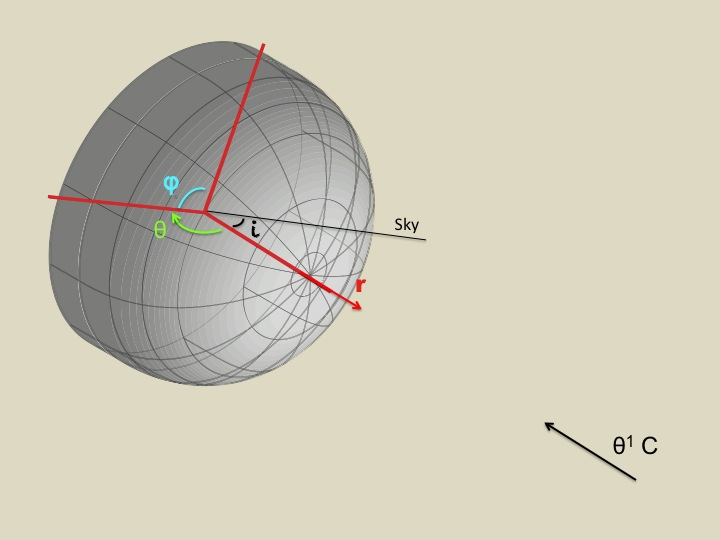
\includegraphics[width=8.5 cm]{./graf_model_3D/geometry_model.jpg}
  \caption{A sketched geometry of the semi-3D model.} \label{fig:3Dgeom}
\end{figure}



%-------------------------------------------------------
\subsection{Radial Density Structure}
\label{sec:density}
%-------------------------------------------------------

As we mentioned above one way to develope models that take into account both, the radiative transfer and the hydrodinamics of the gas, is to introduce an aproximate hydrodinamics in the radiative models that are availables and such are stables. This is our case and the way to introduce the hydrodinams of the gas is using the electron density structure that is a result of the hydrodinamic teorical models.

We divide the proplyd flow into two zones:

\begin{itemize}
  \item{$\rm r > r_0$: An outer, fully ionized flow.}
    \item{$\rm r < r_0$: An inner, partially ionized flow.}
\end{itemize}

This is equivalent to say that the behavior of the physical conditions are diferent in both zones. We suppose that the flow in the partially ionized zone, that correspond to the thin ionization front, is a subsonic flow. This is acelerated to be a supersonic flow in the outer fully ionized zone. The boundary between them are exactly the sonic point. The conditions there, and in every point of the proplyd, are fixed by continuity, it means that the electron density change as the gas-phase velocity change and visceversa. 

\begin{equation}
  \rm n_e(X) = \left\lbrace
    \begin{array}{l}
      f_1(X) \;\;\;\;\; 1 \ge X \ge 0.98 \\
      f_2(X) \;\;\;\;\;  0.02 \ge X \le 0.98  \\
    \end{array}
  \right.
\end{equation}

%-------------------------------------------------------
\subsubsection{The outer zone}
\label{sec:outer}
%-------------------------------------------------------

This is similar to what Will did in \citep{2002ApJ...566..315H}

In the outer zone we assume an isothermal, supersonic, complite
ionized flow. From mass conservation, in spherical geometry and In the
steady state, radial velocity of the ionized gas, $v(r)$

Gas velocity is given by Dyson solution \citep{1968Ap&SS...1..388D}

\begin{equation}
  R = U^{(-1/2)} exp \left [ \frac{1}{4} \left (U^2 -1 \right )
  \right ]
\end{equation}

where $\rm U(R) = v / c_0$ with $v(R)$ is the gas velocity and
$\rm c(R)$ is the sound speed wich is calculated {\it in situ} by Cloudy
for each step.
Due we can not have an analytic solution for U as a function of R,
from this equation generate a table of values for U and R and
interpolate this table for each R that is necesary in the Cloudy model.

At each point the density is calculated by the continuity equation:

\begin{equation}
  \rho (R) = \rho (R_{max}) \left ( \frac{U(R_{max})}{U (R)} \right )
    \left ( \frac{R_{max}}{R} \right ) ^2
\end{equation}

%-------------------------------------------------------
\subsubsection{The boundary}
\label{sec:boundary}
%-------------------------------------------------------

Because the gas velocity is the property that determines the behavior
of other physical properties of the proplyd, the logical boundary
between the regions is exactly the sonic point.

This point is also where the criterion of Stromgren for a density
bounded region is met. That is, where the photoionization balance is
broken and the recombination start to overcome the photoinization.

INSERTAR LA ECUACION

$\rm r = r_0$

$\rm X_H \simeq 0.99$

$u = c$ by definition of the boundary

$c = c_{max}$ at least a local maximum 

%-------------------------------------------------------
\subsubsection{The inner zone}
\label{sec:inner}
%-------------------------------------------------------

Partially ionized region: Density is function of sound speed

In this zone, we follow the simplified analytic model for weak--D
ionization front described in Appendix of the
\citet{2005ApJ...621..328H} paper. Even when this model is for a
plane-parallel ionization front (the momentum conservation assumes
plane parallel geometry) and this is not our case (we have an
divergent geometry) this is an aproximation that could give us a good idea
of the advection effects on the I-front.

Following the A8 equation, 
\begin{equation}
  c(X) = c_m \left [ \frac{T(X)}{T_m} \frac{1+X}{1+X_m}\right]^{1/2}
\end{equation}
If we see the electronic temperature behavior for the waek--D
solutions, Fig.18 from \citet{2005ApJ...621..328H}, we can see that
the temperature could be assume constant in first aproximation, at
least in $0.25 \le X \le 1.0$. This is our case, then the sound speed
will be:
\begin{equation}
  c(X) = c_m \left [ \frac{1+X}{1+X_m}\right]^{1/2}
\end{equation}

As in the Cloudy models the temperature is one of the physical
quantities that are calculated in each zone, we can not use
it for calculate the sound speed in each zone. Then, we made
an aproximation for the behavior of $X$ in the recombination zone, for
calculate the sound speed. We aproximate the H ionization fraction by
a function of \R:

\begin{equation}
  \rm ifrac = 0.5 (tan h (x) + 1.0)
\end{equation}

where $x = x_0 \frac{R + dR -1.0}{dR}$. $x_0$ is where the H
ionization fraction is 0.99, i.e. in the sonic point where $R = 1$ ($ifrac_m = 0.5
(tan h (x_0) + 1.0)$).

Making use of the Mach number $M = v/c$ and the fact of $c_m/c =
\frac{1}{2} \left ( M + M^{-1} \right)$. Then, once more by
continuity, the electronic density in this zone is:
\begin{equation}
  \rho = \rho_m / 1.0 - \sqrt{ 1.0 - \left [ \frac{1+X}{1+X_m} \right ]}
\end{equation}
in contrast to the static case where the density is: $\rho \sim 1/c^2$

%--------------------------------------------------------
\section{Results and Predictions}
\label{sec:results}
%--------------------------------------------------------



%--------------------------------------------------------
\subsection{Physical properties}
\label{sec:physical}
%--------------------------------------------------------

\begin{itemize}
  \item{Electron Density: It has an almost constant increase reaching
      the maximum value in the i-front (after the sonic point) where the H is partially
      ionized. In this zone, the electron density reach the critical
      electron density for some ions, making the collisional
      deexitation a process that need to take into account.\\
    This could be negligible in the outer parts of the flow since they
    are highly ionized, which means that \oiii is the dominant
    coolant. The critical density of this ion is about 1e6 cm-3, which
  is reached just near of the sonic point, that is, where the \oiii
  emission is less than the 10\% of the total \oiii emission. (See Sect.~\ref{sec:emi}).
}
  \item{Temperature: The electron temperature is almost constant in
      the outer zone. As we approache to the He recombination front
      the Te increase reaching the maximum value just before the
      i-front, where the He is neutral and the H still fully ionized. \\
    It is due for two reasons: The first one is that as the radiation
    field goes into the gas-phase of the proplyd, the less energy
    photons are absorved. This cause a hardening of the radiation
    field increasing the mean electron kinetic energy. That is,
    increasing the photoelectric heating per recombination. The second
  one is the electron density increase. It causes collisional
  deexcitation of the main cooling lines.
}
\end{itemize}

%--------------------------------------------------------
\subsection{Ionization structure}
\label{sec:ionization}
%--------------------------------------------------------



%--------------------------------------------------------
\subsection{Emissivities}
\label{sec:emi}
%--------------------------------------------------------

All the high ionization lines are all wholly outside the sonic point.

\neii, \ha, \nii and \oii have almost the 90\% of their emission
in the supersonic zone and the 10\% in the sub-sonic zone.

\sii is about 70\% outside the sonic point and 30\% inside.

\oi is about 20\% outside and 80\% inside the sonic point.

So if we take into account the full emission of the proplyd, and the
sub-sonic zone is not well modelated, the efect of this should be not
very important since it is only going to affect two
lines. Nevertheless, if we want to compare the model predictions with
observations that takes only a little aperture of the proplyd and it
is near of the center (near the i-front), the sub-sonic zone will be
very important.

There are a clear separation of 3 km/s (about 15\%) between the median
velocity of the \oiii 5007 and 4363 lines.

Discutir tambien la diferencia que hay entre la linea auroral y la
nebular de \nii para ver la importancia de las desexitaciones
colisionales. Una es mas afectada que la otra y por lo tanto conforme
vamos a las zonas de mayor densidad la razon entre ellas debe ir
cambiando, aumentando de hecho.

%--------------------------------------------------------
\section{Conclusion}
\label{sec:conclusions}
%--------------------------------------------------------

We will construct Cloudy models of a series of individual radial cuts from the center of the proplyd, at different angles $\theta$ from the proplyd axis.

\bibliographystyle{t}

\bibliography{model}

\end{document}
